\subsection{Use Case for applying \cbc}

``Router'' use case exposes an example of a simple Router component with configured quality of service (QoF) management, which is used in telecommunication networks. In this use case Stakeholders have provided the system requirements as a text document with semi-structured information and a simple component diagram (Figure~\ref{fig:route}). 
\begin{center}
\textbf{\textit{\scriptsize System requirements.}}
\end{center}

\scriptsize``In communication system Data Link (DL) is usually used by several users. The users can proceed with different types of traffic. For better use of Data Link resources, traffic from diverse users can differ by priorities (depends on QoS and user's agreement). Depending on the priority, traffic should be forwarded along a certain route with a defined latency. For high priority packets the route shall be defined with the lowest latency. The lower priority of traffic, the higher latency the provided route has. Configuration input for Selector should be specified by QoS agreement of user.

Message Filter defines priority of packets and send them directly to Selector. 

Selector should:
\begin{itemize}
	\item receive packets from Message Filter;
  \item define a proper route, according to packet priority;
\end{itemize}

Packets shall be sent from Selector to Data Link using 3 routes.

All QoS policy is defined in Selector component. 

There are 3 data priorities: 
\begin{enumerate}
	\item High priority information - Selector should route such packets into 1st route only! 
  \item	Middle level priority - packets can be sent by Selector into 1st route , if the route is free; otherwise, traffic is transmitted into 2nd route;
  \item	Low priority - data can be sent in 3 routers, depends on which route is free at the moment.''
\end{enumerate}

\begin{figure}[!t]
\centering
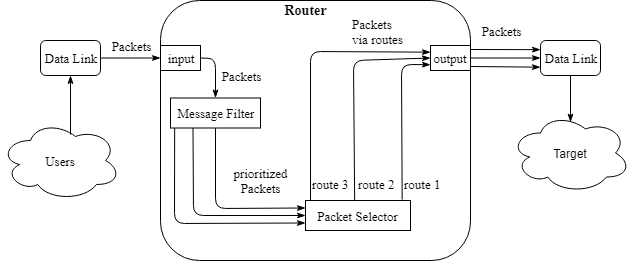
\includegraphics[width=3.5in]{use_case/router.png}
\caption{Diagram of the Router in the Network}
\label{fig:route}
\end{figure}

\normalsize
\subsubsection{Requirements Structuring}
\\
Initial phase of development process is elicitation and analysis of requirements. We claim, that during analysis process \asp should be applied to the requirements in order to categorize them and form their structure. Considering further the ``'Router' use case, the following \asp can be assigned to the given requirements:\\

\scriptsize Req-1.	In communication system Data Link is usually used by several users. 
\begin{description}
	\item[\normalsize \textit{Mode aspect} implies, that DL is in active state, when the] 
	\item[\normalsize users send traffic]
\end{description}\\

\scriptsize Req-2.	The users can proceed with different types of traffic. 
\begin{description}
	\item[\normalsize \textit{Signal aspect} describes, that the packets have different] 
	\item[\normalsizetypes] 
\end{description}\\

\scriptsize Req-3.	For better use of Data Link resources, traffic from diverse users can differ by priorities (depends on QoS in user's agreement). 
\begin{description}
	\item[\normalsize \textit{Signal aspect} describes the traffic] 
\end{description}\\

\scriptsize Req-4.	Depending on the priority, traffic should be forwarded along a certain route with a defined latency. 
\begin{description}
  \item[\normalsize \textit{Parameter definition aspect} indicates, that priorities,] 
	\item[\normalsize routes and latency can be kept as re-useable parameters] 
	\item[\normalsize \textit{Signal aspect} describes input for the routes] 
	\item[\normalsize \textit{Functional aspect} describes behavior of Packets Selector] 
	\item[\normalsize \textit{Temporal property aspect} shows, that the statement] 
	\item[\normalsize includes a condition]  
\end{description}\\

\normalsize and continue with other requirements in same way.

\scriptsize Req-5.	For high priority packets the route shall be defined with the lowest latency. 

\normalsize
(Functional aspect � describes a behaviour of Selector

, Temporal property aspect � here describes a condition for high priortiy ptaffic ,

 Signal aspect � describes traffic)

\scriptsize Req-6.	The lower priority of traffic, the higher latency the provided route has. 

\normalsize
(Functional aspect � describes a behaviour of Selector

, Temporal property aspect � here describes a condition for high priortiy ptaffic ,

 Signal aspect � describes traffic)

\scriptsize Req-7.	Configuration input for Selector should be specified by QoS agreement of user.

\normalsize
(, Temporal property aspect � here describes a condition for high priortiy ptaffic ,

Parameter definition aspect � parameters for input can be reusable)

\scriptsize Req-8.	Message Filter defines priority of packets and send them directely to Selector. 

\normalsize
( Functional aspect � describes a behaviour of Message Filter

Signal aspect � pints that packets are prioritized, 

Mode aspect � comes from here that MF is active only if users send traffic, in other way the system in inactive mode )

\scriptsize Req-9.	Selector should:

�	 receive packects from Message Filter;

�	define a proper route, according to packet priority;

\normalsize
( Functional aspect � describes behaviour of the Selector

, Temporal property aspect � �according to � expose that the statement includes some information about condition for sending packets

Parameter definition aspect) � routes, priorities can be reusable parameters , their values can be changed.

\scriptsize Req-10.	Packets shall be sent from Selector to Data Link using 3 routes. � 

\normalsize
Signal aspect � describes packets 

 Functional aspect � describes beheviour of Selector

Parameter definition aspect � the requirements gives number of routes, which can be changed in anther system and routes can be reused.

\scriptsize Req-11.	All QoS policy is defined in Selector component. 

\normalsize
Functional aspect � implies that Selector has specified behaviour according to QoS policy.

\scriptsize Req-12.	There are 3 data priorities: 

�	High piority information � Selector should route such packes into 1st route only! 

�	Midel level priority � packets can be sent by Selector into 1st route , if the route is free; otherwise, traffic is transmitted into 2nd route;

�	Low priority � data can be sent in 3 routers, depends on which route is free at the moment.

\normalsize
 Temporal property aspect � policy description

Parameter definition aspect � priorities and routes can be reused

Functional aspect � here defines a behaviour of the Selector \\

Now, when the requirements have been categorized, the requirements engineer can proceed with preliminary inspection. First of all, he/she should check, if all requirements have \asp. Next, re-consider the requirements with more than 1 aspect in their categorization; it can mean, that such requirements are not precise enough. For example, the requirement ``Req-4'':  

\scriptsize Req-4. ``Depending on the priority, traffic should be forwarded along a certain route with a defined latency.``

\normalsize
(Parameter definition aspect � the requirement defines a parametric value. This allows to reused other requirements by changing the value of the parameter � for priorities, routes and latency description

, Functional aspect - the requirement specifies a particular behavior by relating inputs and outputs � describes inputs for the routes

, Signal aspect - the requirement defines a signal, its type and its range � to describe the traffic)

Temporal property aspect - the requirement defines a property, which can be defined using temporal patterns � �depends� points to conditions of the statement
\\
It can be splitted into several requirements according to categories reflected by aspects:

Based on Functional aspect :

\scriptsize Req-4.1.	 Selector should forward traffic along a certain route. 

\normalsize
From Parameter definition aspect:

\scriptsize Req-4.2.	 Every route operates with defined latency.

Req-4.3.	There are several (three) routes.

Req-4.4.	There are several priorities for traffic.

\normalsize
From Signal aspect

\scriptsize 4.1.	Traffic is prioritized. 

\normalsize
From Temporal property aspect:

\scriptsize Req-4.2.	Traffic priority defines a route for traffic.\\

\normalsize
The ideal case is when every requirement has only one aspect, but in real project requirements categories usually overlap each other. Therefore, number of \asp attached to a requirement should tend to be minimized. \\

After applying this method to other requirements, we have received the following structure of requirement:

\scriptsize 
Req-1.	 In communication system Data Link is usually used by several users. (Functional aspect)

Req-2.	The users can proceed with different types of traffic. (Signal aspect)

Req-3.	For better use of Data Link resources, traffic from diverse users can differ by priorities (depends on QoS in user�s agreement). (Signal aspect)

Req-4.1	 Selector should forward traffic along a certain route. (Functional aspect)

Req-4.2	Every route operates with defined latency.(Parameter definition aspect)

Req-4.3	There are several (three) routes. (Parameter definition aspect)

Req-4.4 There are several priorities for traffic. (Parameter definition aspect)

Req-4.5	Traffic is prioritized. (Signal aspect)

Req-4.6	Traffic priority defines a route for traffic. (Temporal property aspect)

Req-5.	For high priority packets the route shall be defined with the lowest latency. (Temporal property aspect)

Req-6.	The lower priority of traffic, the higher latency the provided route has. (Temporal property aspect)

Req-7.	Configuration input for Selector should be specified by QoS agreement of user. (Signal aspect)

Req-8.1	Message Filter defines priority of packets. (Functional aspect)

Req-8.2 Message Filter sends packets directly to Selector. (Functional aspect)

Req-9.1	Selector should receive packets from Message Filter; (Functional aspect)

Req-9.2	Selector should define a proper route, according to packet priority; (Functional aspect and Temporal property aspect)

Req-10.1	Selector shall send packets to Data Link. (Functional aspect and Signal aspect)

Req-10.2	Selector shall use 3 routes for packets sending to Data Link. (Functional aspect)

Req-10.3	There are 3 routes for sending packets from Selector to Data Link. (Parameter definition aspect)

Req-11	All QoS policy is defined in Selector component. (Functional aspect)

Req-12.1	There are 3 data priorities (Parameter definition aspect)

Req-12.2.	High piority information � Selector should route such packes into 1st route only! (Temporal property aspect)

Req-12.3.	Midel level priority � packets can be sent by Selector into 1st route , if the route is free; otherwise, traffic is transmitted into 2nd route; (Temporal property aspect)

Req-12.4.	Low priority � data can be sent in 3 routers, depends on which route is free at the moment. (Temporal property aspect)

\\
\normalsize
Now we have more consistent high-level requirements in comparison with initially provided requirements by stakeholder. That means, the requirements are better structured, more precise and less complex. These characteristics rise quality of the requirements. Therefore, it is easier to work with such requirements during development phase or review process.


These structured HLR now can be an input for system design process. Developers can also analyze the requirements and provide requirements inferred from HLR. (see in paper) � desing choice aspect.
\\
....
\\
